% Created by tikzDevice version 0.12.3.1 on 2020-07-05 11:02:12
% !TEX encoding = UTF-8 Unicode
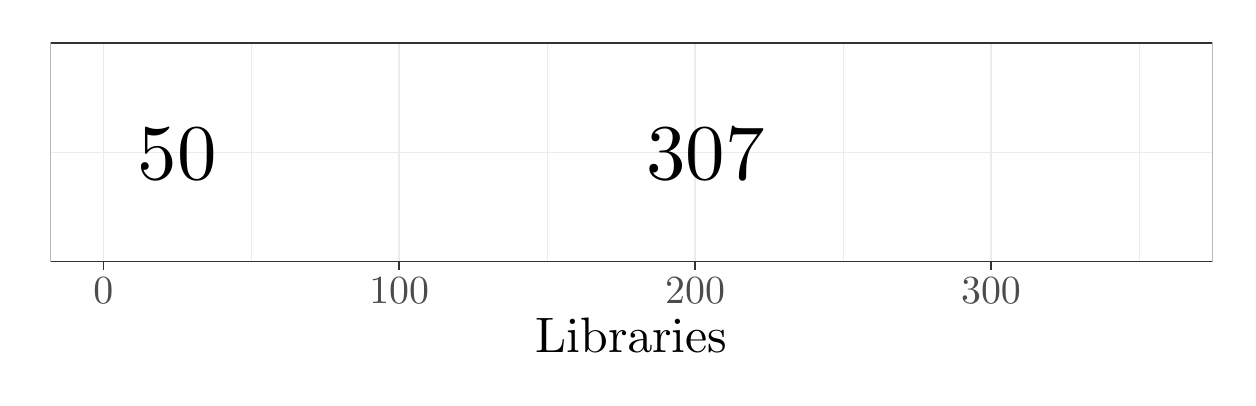
\begin{tikzpicture}[x=1pt,y=1pt]
\definecolor{fillColor}{RGB}{255,255,255}
\path[use as bounding box,fill=fillColor,fill opacity=0.00] (0,0) rectangle (433.62,126.47);
\begin{scope}
\path[clip] (  0.00,  0.00) rectangle (433.62,126.47);
\definecolor{drawColor}{RGB}{255,255,255}
\definecolor{fillColor}{RGB}{255,255,255}

\path[draw=drawColor,line width= 0.6pt,line join=round,line cap=round,fill=fillColor] (  0.00,  0.00) rectangle (433.62,126.47);
\end{scope}
\begin{scope}
\path[clip] (  8.25, 41.81) rectangle (428.12,120.97);
\definecolor{fillColor}{RGB}{255,255,255}

\path[fill=fillColor] (  8.25, 41.81) rectangle (428.12,120.97);
\definecolor{drawColor}{gray}{0.92}

\path[draw=drawColor,line width= 0.3pt,line join=round] ( 80.79, 41.81) --
	( 80.79,120.97);

\path[draw=drawColor,line width= 0.3pt,line join=round] (187.71, 41.81) --
	(187.71,120.97);

\path[draw=drawColor,line width= 0.3pt,line join=round] (294.63, 41.81) --
	(294.63,120.97);

\path[draw=drawColor,line width= 0.3pt,line join=round] (401.55, 41.81) --
	(401.55,120.97);

\path[draw=drawColor,line width= 0.6pt,line join=round] (  8.25, 81.39) --
	(428.12, 81.39);

\path[draw=drawColor,line width= 0.6pt,line join=round] ( 27.34, 41.81) --
	( 27.34,120.97);

\path[draw=drawColor,line width= 0.6pt,line join=round] (134.25, 41.81) --
	(134.25,120.97);

\path[draw=drawColor,line width= 0.6pt,line join=round] (241.17, 41.81) --
	(241.17,120.97);

\path[draw=drawColor,line width= 0.6pt,line join=round] (348.09, 41.81) --
	(348.09,120.97);

\path[] ( 27.34, 51.71) rectangle ( 80.79,111.08);

\path[] ( 80.79, 51.71) rectangle (409.03,111.08);
\definecolor{drawColor}{RGB}{0,0,0}

\node[text=drawColor,anchor=base,inner sep=0pt, outer sep=0pt, scale=  2.85] at ( 54.06, 71.60) {50};

\node[text=drawColor,anchor=base,inner sep=0pt, outer sep=0pt, scale=  2.85] at (244.91, 71.60) {307};
\definecolor{drawColor}{gray}{0.20}

\path[draw=drawColor,line width= 0.6pt,line join=round,line cap=round] (  8.25, 41.81) rectangle (428.12,120.97);
\end{scope}
\begin{scope}
\path[clip] (  0.00,  0.00) rectangle (433.62,126.47);
\definecolor{drawColor}{gray}{0.20}

\path[draw=drawColor,line width= 0.6pt,line join=round] ( 27.34, 39.06) --
	( 27.34, 41.81);

\path[draw=drawColor,line width= 0.6pt,line join=round] (134.25, 39.06) --
	(134.25, 41.81);

\path[draw=drawColor,line width= 0.6pt,line join=round] (241.17, 39.06) --
	(241.17, 41.81);

\path[draw=drawColor,line width= 0.6pt,line join=round] (348.09, 39.06) --
	(348.09, 41.81);
\end{scope}
\begin{scope}
\path[clip] (  0.00,  0.00) rectangle (433.62,126.47);
\definecolor{drawColor}{gray}{0.30}

\node[text=drawColor,anchor=base,inner sep=0pt, outer sep=0pt, scale=  1.44] at ( 27.34, 26.95) {0};

\node[text=drawColor,anchor=base,inner sep=0pt, outer sep=0pt, scale=  1.44] at (134.25, 26.95) {100};

\node[text=drawColor,anchor=base,inner sep=0pt, outer sep=0pt, scale=  1.44] at (241.17, 26.95) {200};

\node[text=drawColor,anchor=base,inner sep=0pt, outer sep=0pt, scale=  1.44] at (348.09, 26.95) {300};
\end{scope}
\begin{scope}
\path[clip] (  0.00,  0.00) rectangle (433.62,126.47);
\definecolor{drawColor}{RGB}{0,0,0}

\node[text=drawColor,anchor=base,inner sep=0pt, outer sep=0pt, scale=  1.80] at (218.18,  9.00) {Libraries};
\end{scope}
\end{tikzpicture}
